\begin{figure}[htpb]
	\capstart{}
	\subfloat[\(\Re\big\{\pixel{Y_{00}}\big\}\)]
	{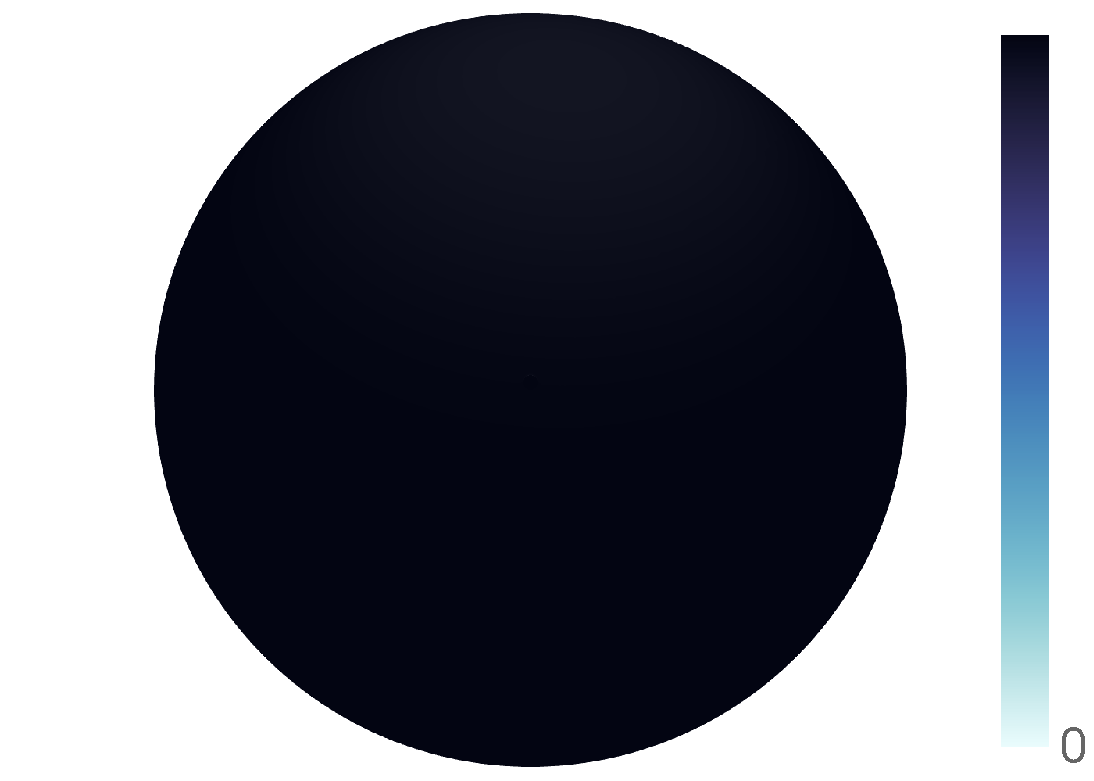
\includegraphics[trim={23 7 3 6},clip,width=.2\textwidth]{spherical_harmonic_0l_0m_L128_real_norm.pdf}}
	\newline
	\subfloat[\(\Re\big\{\pixel{Y_{10}}\big\}\)]
	{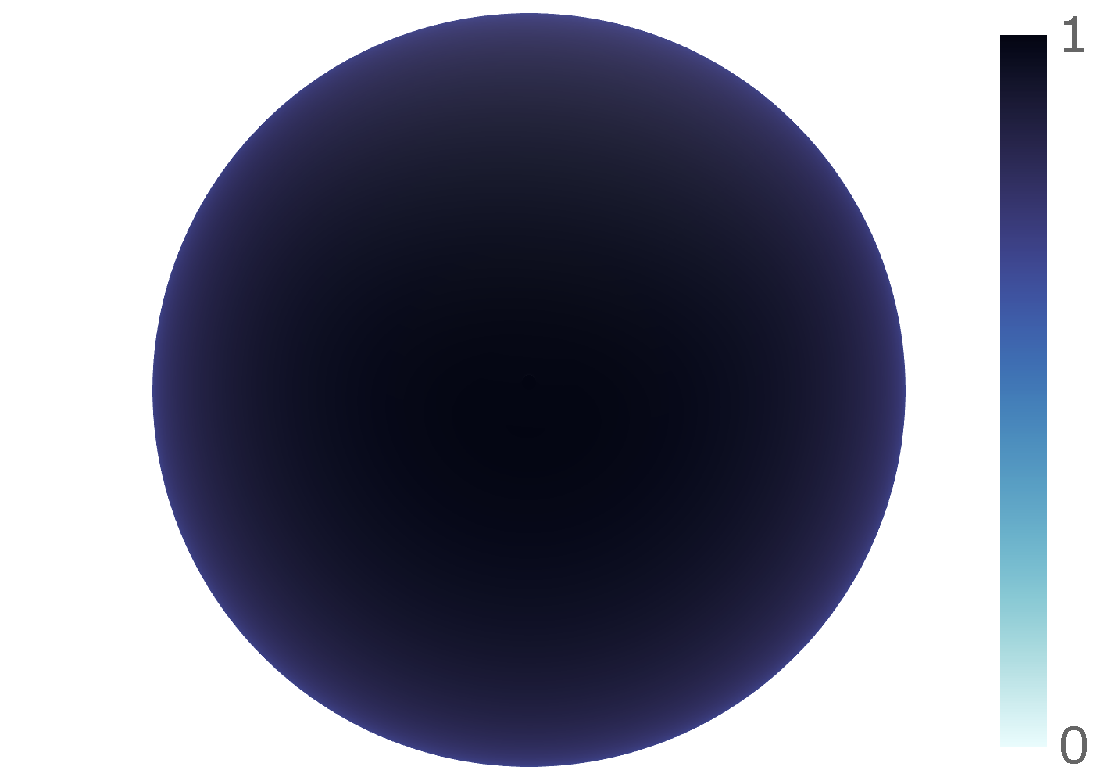
\includegraphics[trim={23 7 3 6},clip,width=.2\textwidth]{spherical_harmonic_1l_0m_L128_real_norm.pdf}}
	%
	\subfloat[\(\Re\big\{\pixel{Y_{11}}\big\}\)]
	{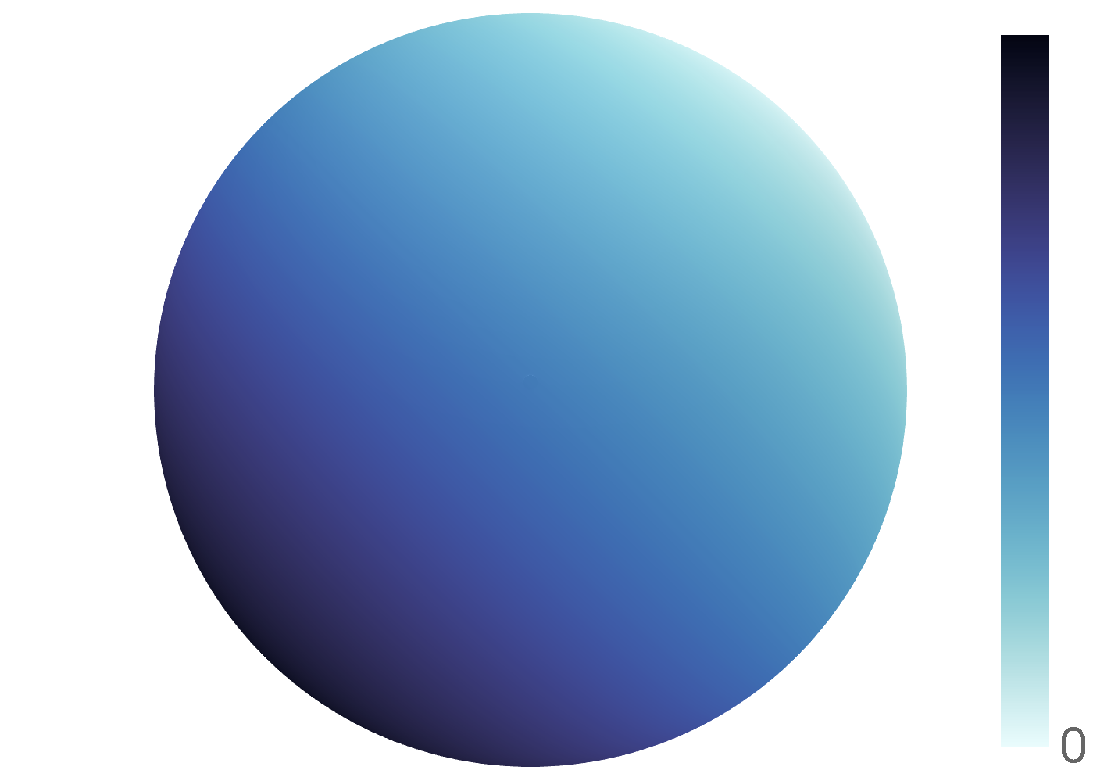
\includegraphics[trim={23 7 3 6},clip,width=.2\textwidth]{spherical_harmonic_1l_1m_L128_real_norm.pdf}}
	\newline
	\subfloat[\(\Re\big\{\pixel{Y_{20}}\big\}\)]
	{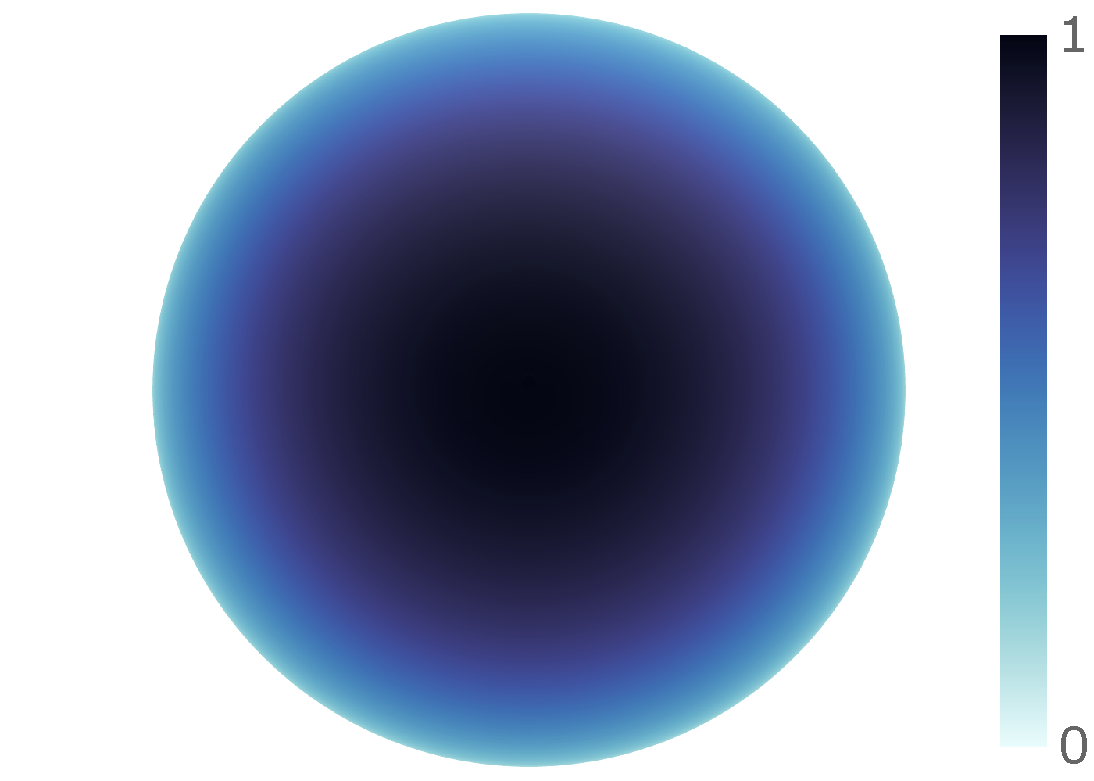
\includegraphics[trim={23 7 3 6},clip,width=.2\textwidth]{spherical_harmonic_2l_0m_L128_real_norm.pdf}}
	%
	\subfloat[\(\Re\big\{\pixel{Y_{21}}\big\}\)]
	{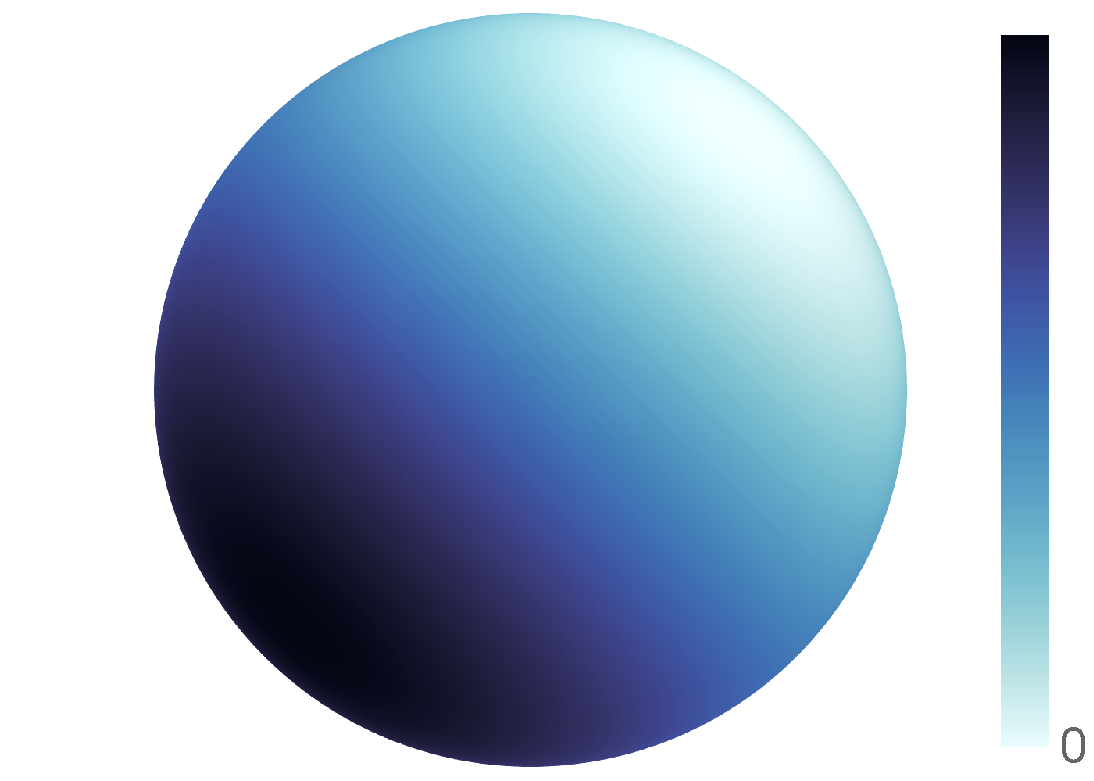
\includegraphics[trim={23 7 3 6},clip,width=.2\textwidth]{spherical_harmonic_2l_1m_L128_real_norm.pdf}}
	%
	\subfloat[\(\Re\big\{\pixel{Y_{22}}\big\}\)]
	{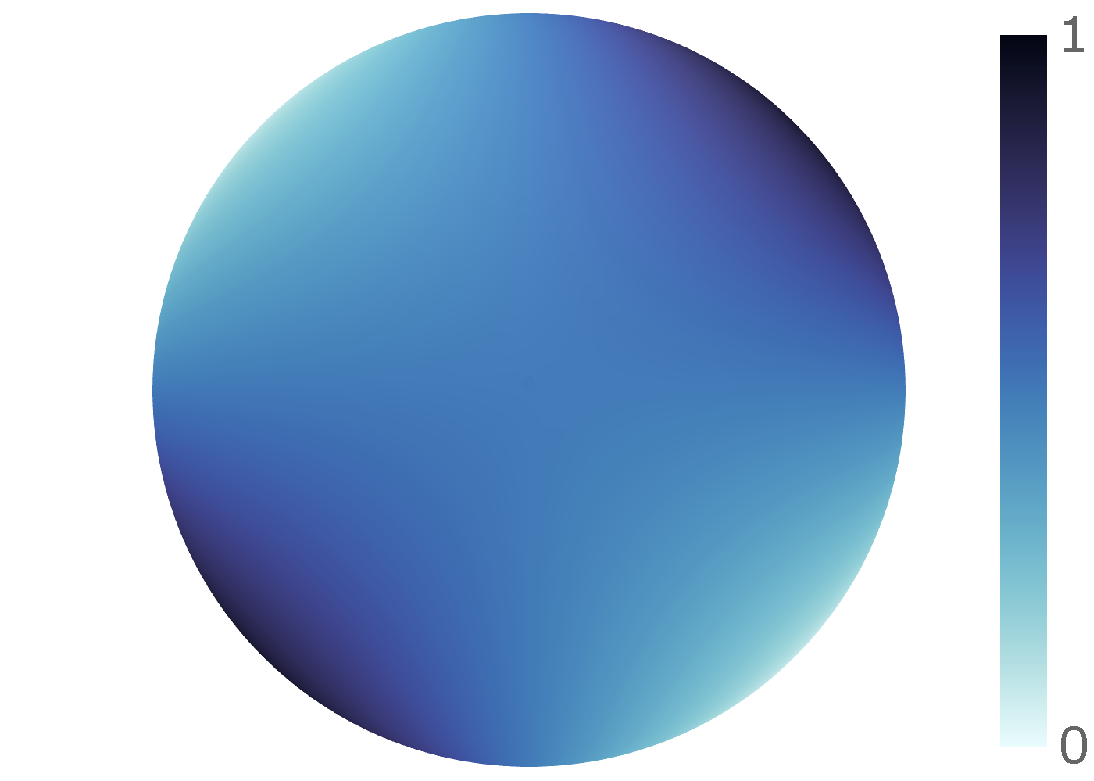
\includegraphics[trim={23 7 3 6},clip,width=.2\textwidth]{spherical_harmonic_2l_2m_L128_real_norm.pdf}}
	\newline
	\subfloat[\(\Re\big\{\pixel{Y_{30}}\big\}\)]
	{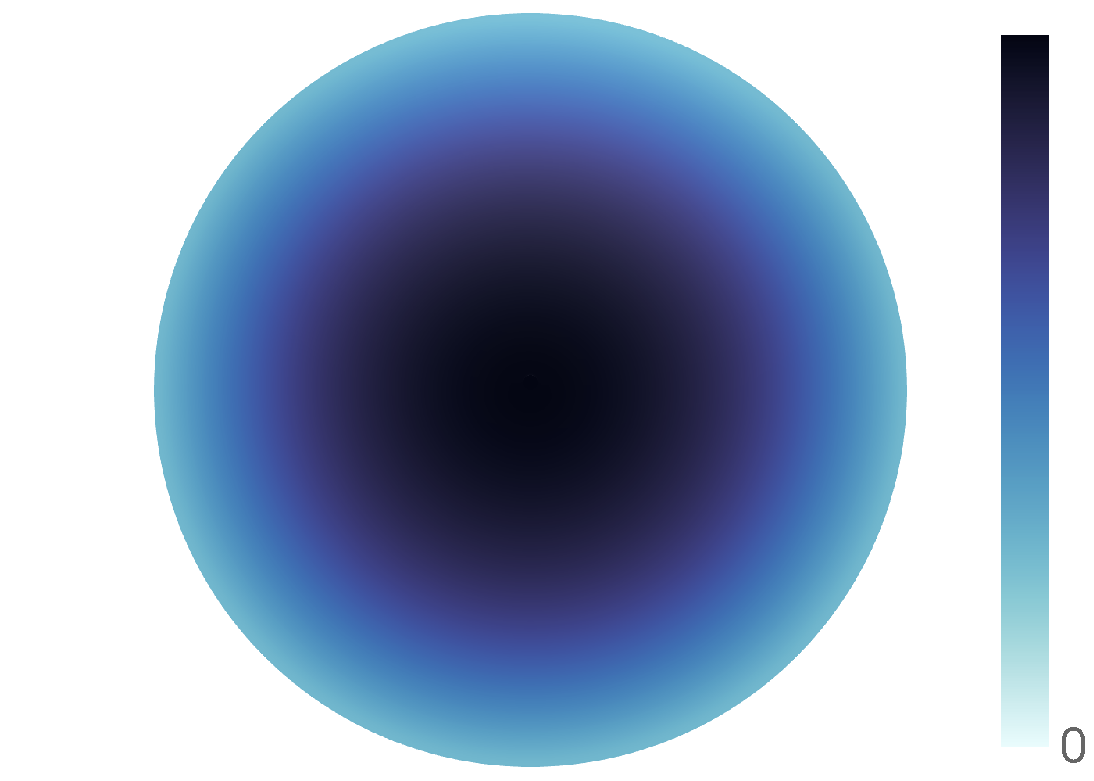
\includegraphics[trim={23 7 3 6},clip,width=.2\textwidth]{spherical_harmonic_3l_0m_L128_real_norm.pdf}}
	%
	\subfloat[\(\Re\big\{\pixel{Y_{31}}\big\}\)]
	{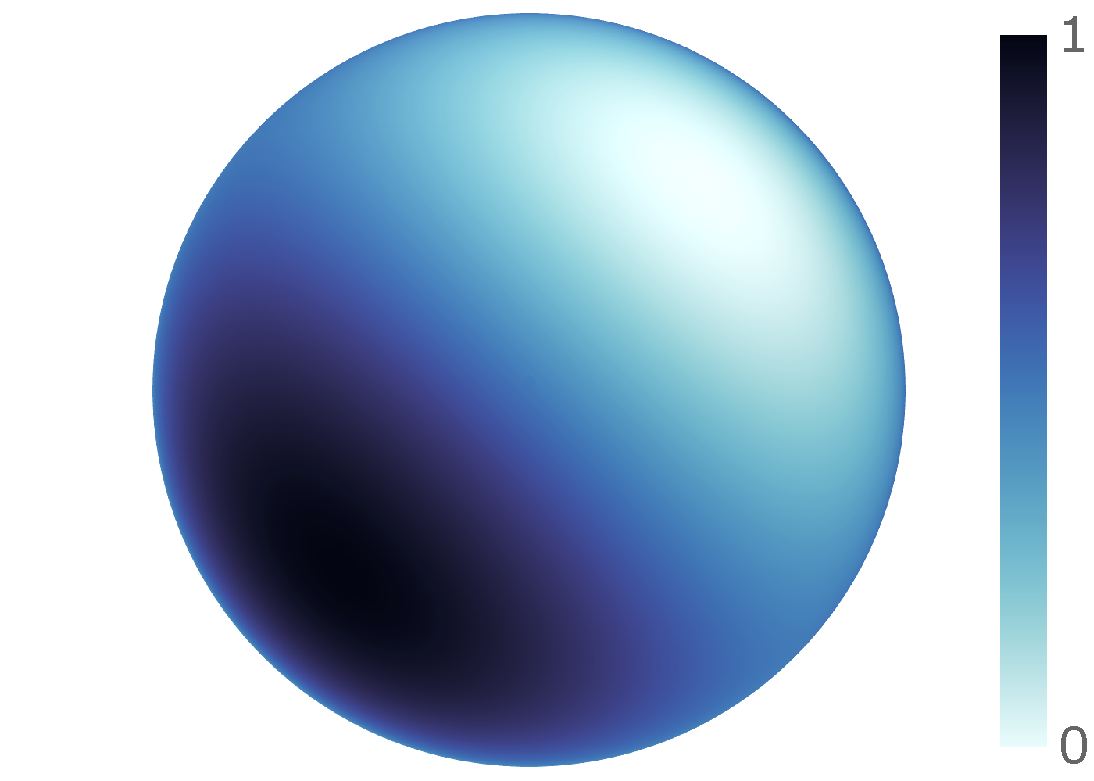
\includegraphics[trim={23 7 3 6},clip,width=.2\textwidth]{spherical_harmonic_3l_1m_L128_real_norm.pdf}}
	%
	\subfloat[\(\Re\big\{\pixel{Y_{32}}\big\}\)]
	{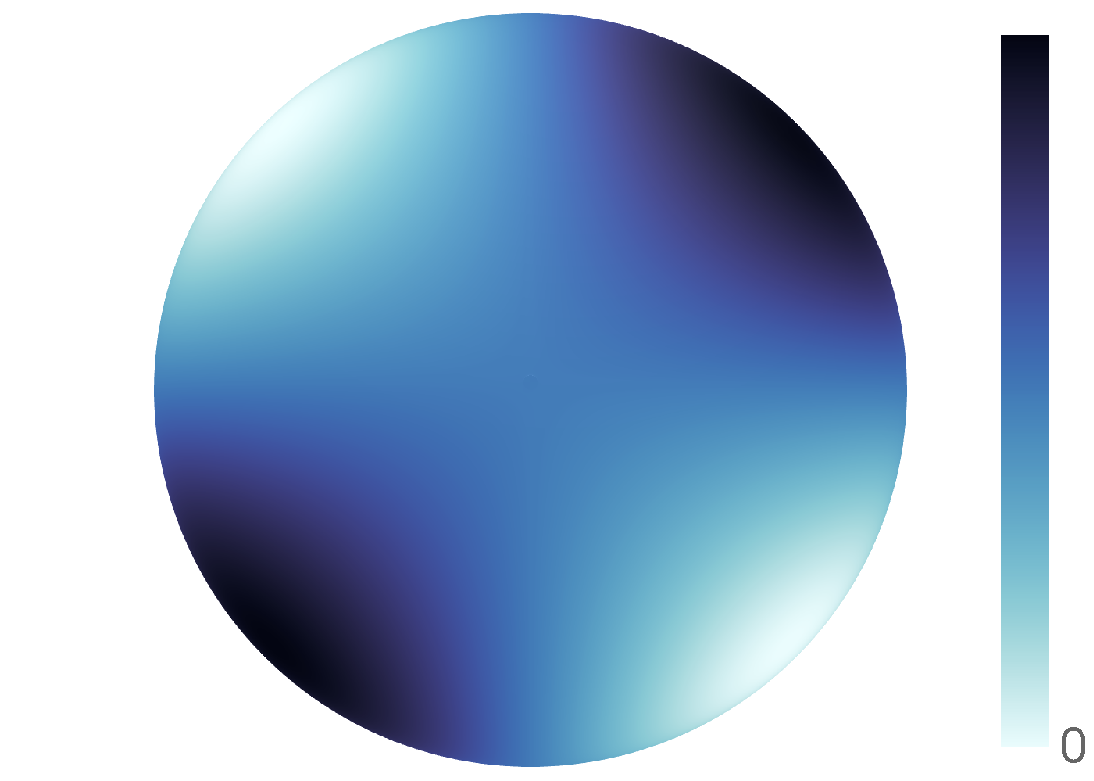
\includegraphics[trim={23 7 3 6},clip,width=.2\textwidth]{spherical_harmonic_3l_2m_L128_real_norm.pdf}}
	%
	\subfloat[\(\Re\big\{\pixel{Y_{33}}\big\}\)]
	{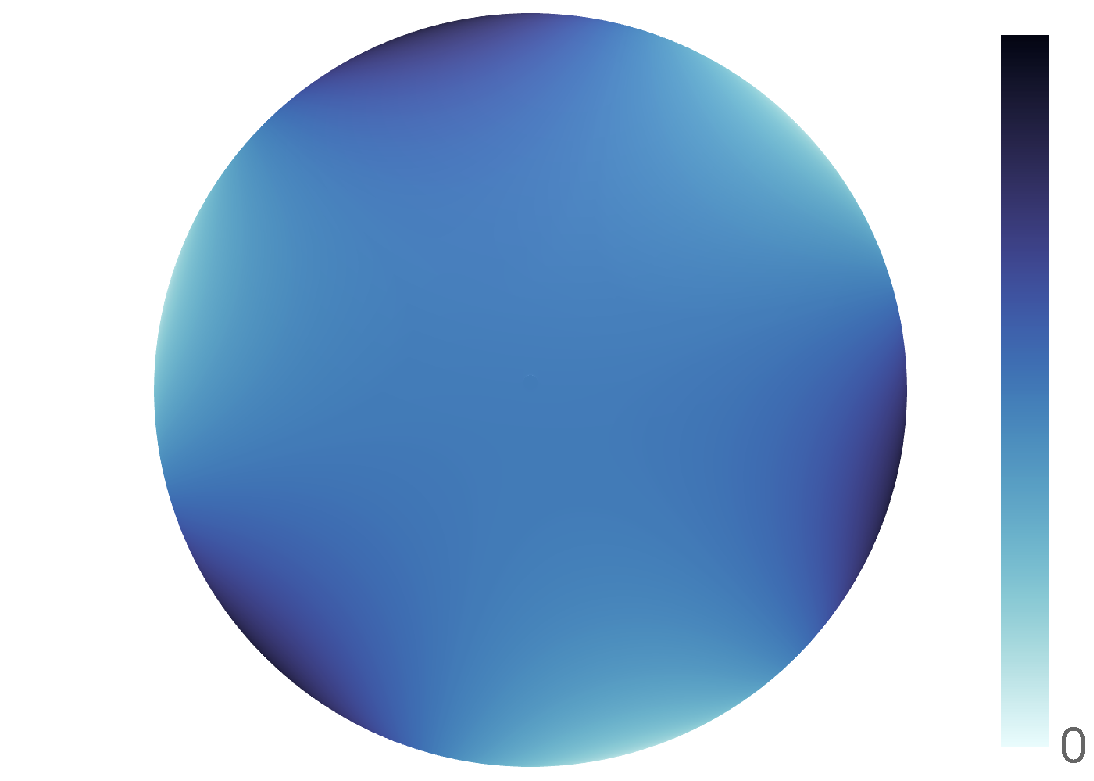
\includegraphics[trim={23 7 3 6},clip,width=.2\textwidth]{spherical_harmonic_3l_3m_L128_real_norm.pdf}}
	\newline
	\subfloat[\(\Re\big\{\pixel{Y_{40}}\big\}\)]
	{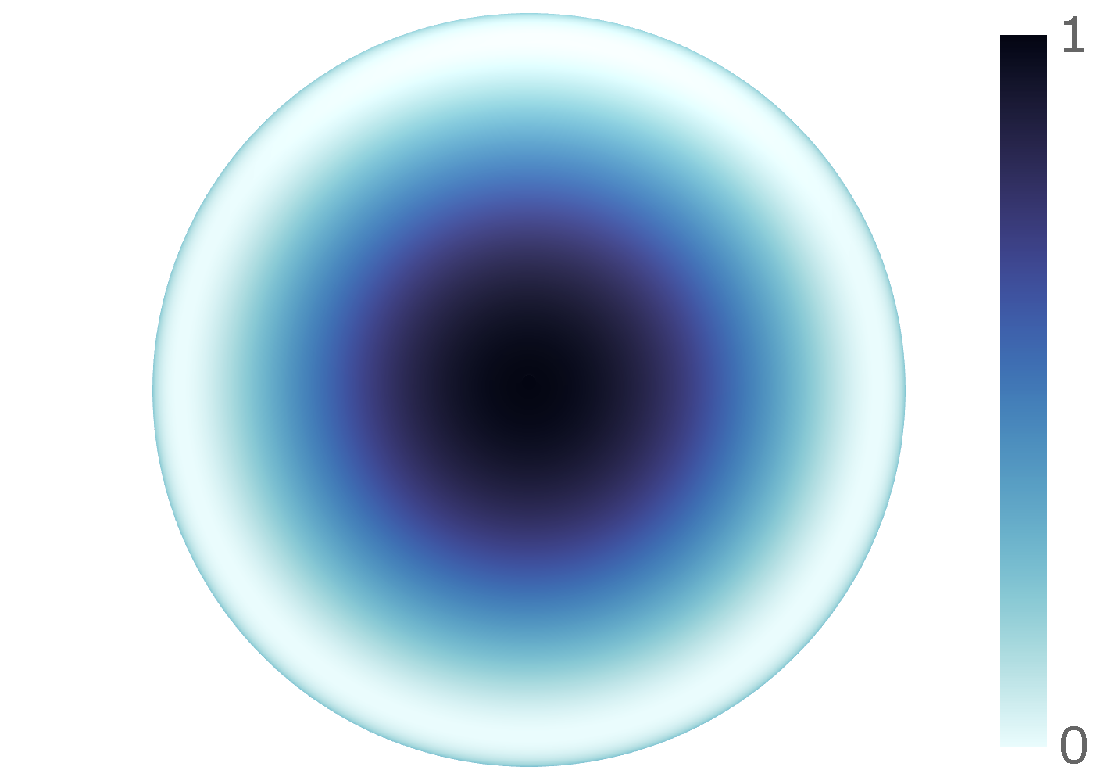
\includegraphics[trim={23 7 3 6},clip,width=.2\textwidth]{spherical_harmonic_4l_0m_L128_real_norm.pdf}}
	%
	\subfloat[\(\Re\big\{\pixel{Y_{41}}\big\}\)]
	{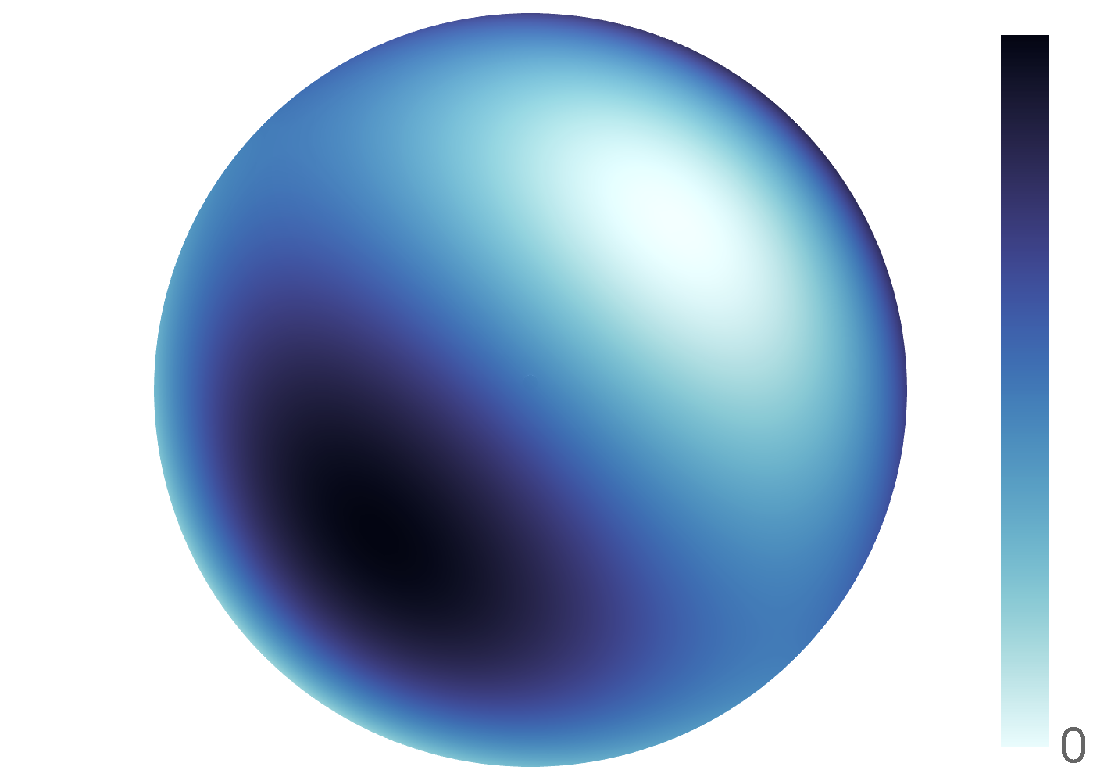
\includegraphics[trim={23 7 3 6},clip,width=.2\textwidth]{spherical_harmonic_4l_1m_L128_real_norm.pdf}}
	%
	\subfloat[\(\Re\big\{\pixel{Y_{42}}\big\}\)]
	{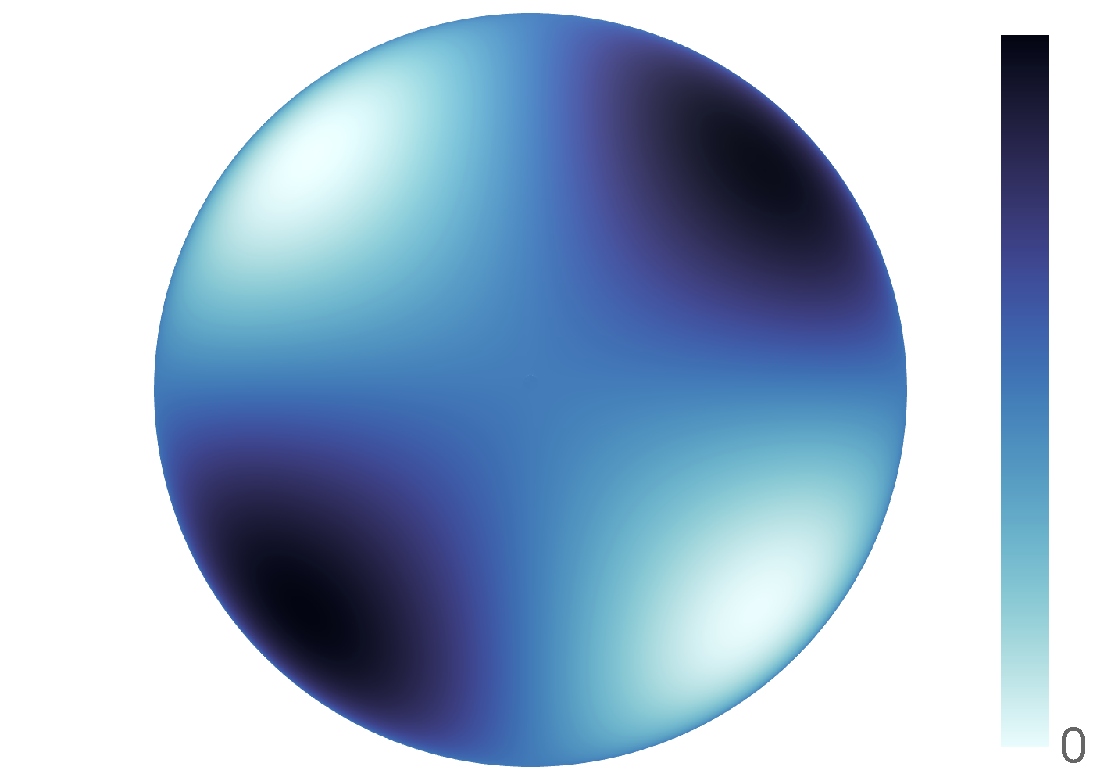
\includegraphics[trim={23 7 3 6},clip,width=.2\textwidth]{spherical_harmonic_4l_2m_L128_real_norm.pdf}}
	%
	\subfloat[\(\Re\big\{\pixel{Y_{43}}\big\}\)]
	{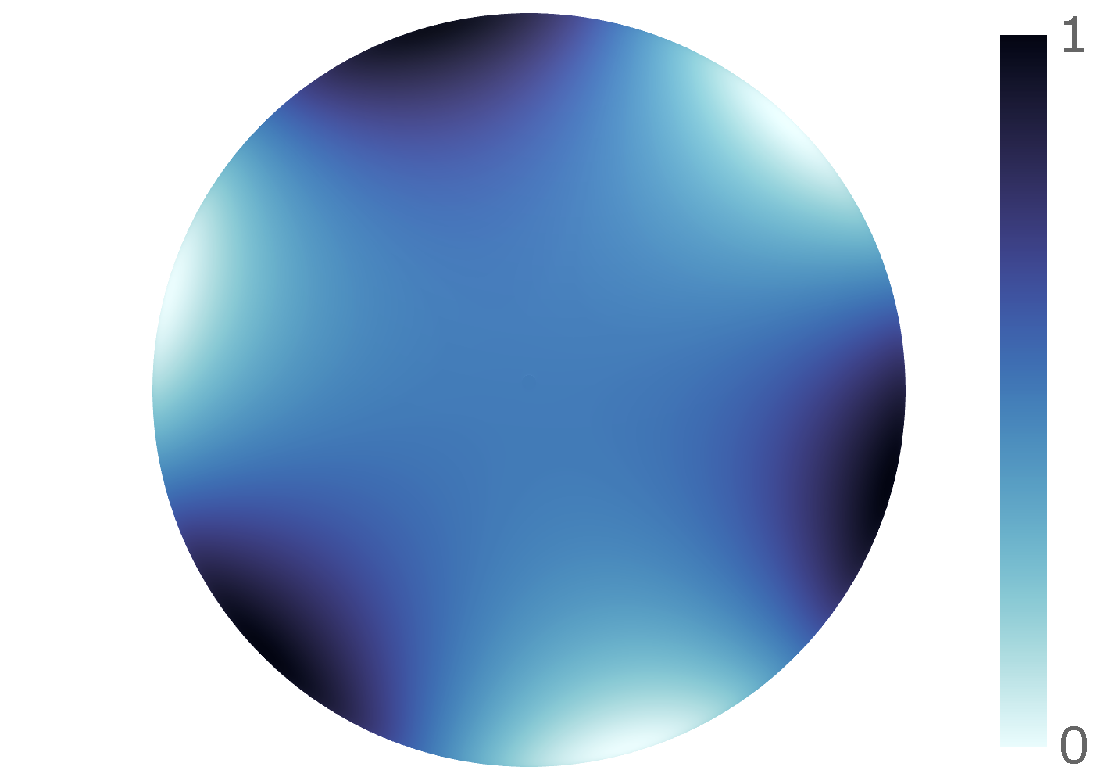
\includegraphics[trim={23 7 3 6},clip,width=.2\textwidth]{spherical_harmonic_4l_3m_L128_real_norm.pdf}}
	%
	\subfloat[\(\Re\big\{\pixel{Y_{44}}\big\}\)]
	{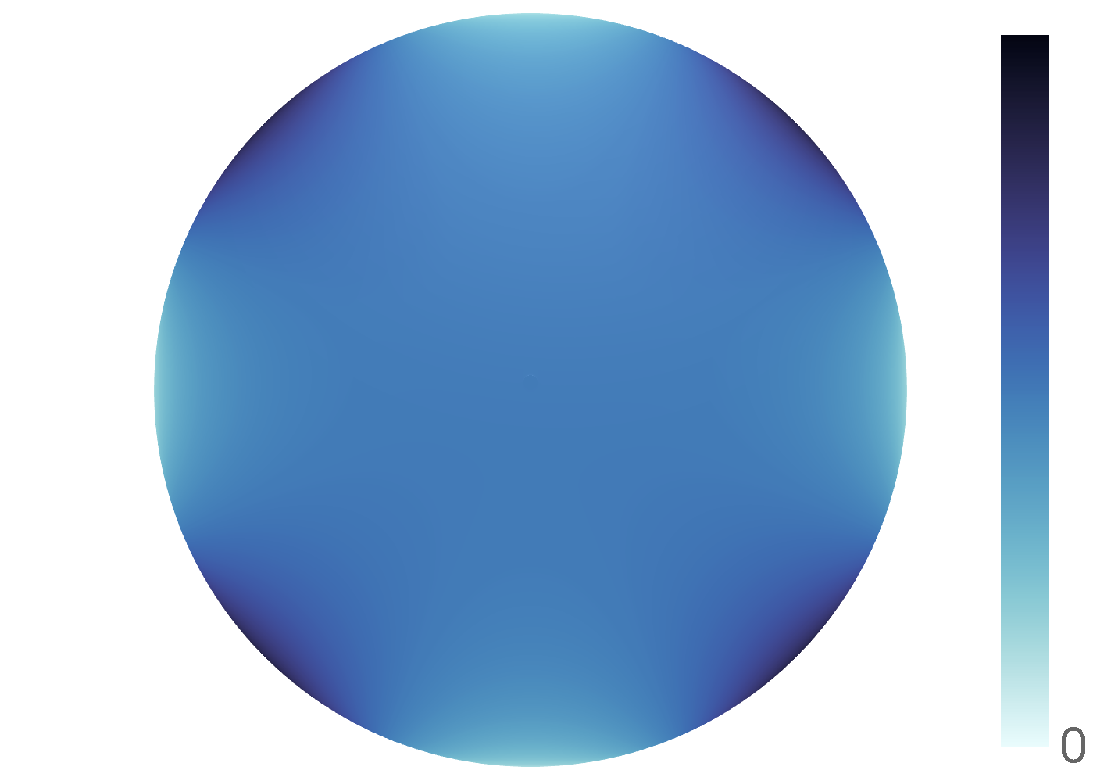
\includegraphics[trim={23 7 3 6},clip,width=.2\textwidth]{spherical_harmonic_4l_4m_L128_real_norm.pdf}}
	\caption[
		The spherical harmonics for \(\ell=0,\ldots,4\)
	]{
		The real part of the spherical harmonics \(\pixel{\harmonic{Y}}\) for \(\ell=0,\ldots,4\) (top-to-bottom) and \(m=0,\ldots,\ell{}\) (left-to-right).
		The negative order harmonics \(\pixel{Y_{\ell(-m)}}\) have not been included as they are simply rotated with respect to the positive order harmonics by \(\SI{90}{\degree}/m\).
	}\label{fig:chapter2_spherical_harmonics}
\end{figure}
